\documentclass[11pt, xcolor=dvipsnames]{beamer}
\usepackage[utf8]{inputenc}
\usepackage[ngerman]{babel}
\usepackage{amsmath}
\usepackage{amsfonts}
\usepackage{amssymb}
\usepackage{graphicx}
\usepackage{listings}
\usepackage{xcolor}
\usepackage{pgfplots}
\usepackage{pgf-pie}
\usetheme{metropolis}
\metroset{block=fill, progressbar=head}
\lstset{
	language        = php,
	basicstyle      = \small\ttfamily,
	keywordstyle    = \color{RoyalBlue},
	stringstyle     = \color{Black},
	identifierstyle = \color{Green},
	commentstyle    = \color{Gray},
	emph            =[1]{php},
	emphstyle       =[1]\color{Black},
	emph            =[2]{if,and,or,else},
	emphstyle       =[2]\color{RoyalBlue},
	showstringspaces=false}

\author{Martin Duschek}
\title{Evolution von Code bei Major-Releases von Programmiersprachen}
\subtitle{am Beispiel der Migration zu PHP7}
\institute{HTWK Leipzig}

\begin{document}
	\maketitle
	
	\begin{frame}{Inhalt}
		\setbeamertemplate{section in toc}[sections numbered]
  		\tableofcontents[hideallsubsections]
	\end{frame}

	\section{Grundlagen}
	\begin{frame}{PHP}
    \begin{figure}
        \centering
        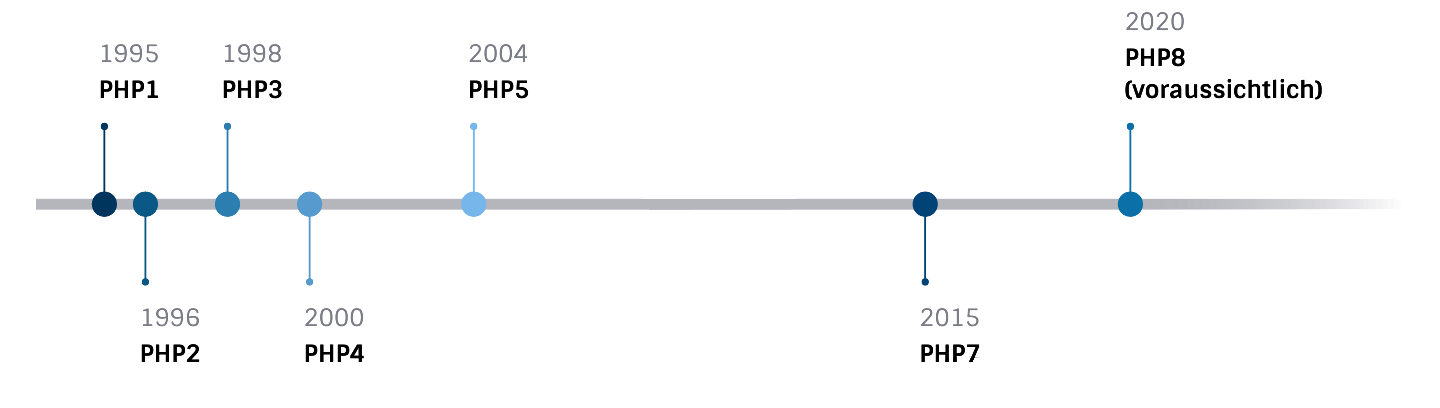
\includegraphics[width=290px]{img/timeline.png}	
        \caption{Major-Releases von PHP im Zeitverlauf}		
    \end{figure}
\end{frame}

\begin{frame}{Versionierung von Software}
    Semantic Versioning \nocite{preston-werner_semantic_nodate}:
    \begin{center}
        \alert{Major.Minor.Patch[-Pre-Release]}
    \end{center}
    \begin{itemize}
        \item \textbf{Major}: inkompatible API-Änderungen
        \item \textbf{Minor}: abwärtskompatible Änderungen oder \emph{Deprecations}
        \item \textbf{Patch}: abwärtskompatible Bugfixes
    \end{itemize}
\end{frame}

\begin{frame}{Versionierung von Software}
    \begin{figure}
        \centering
        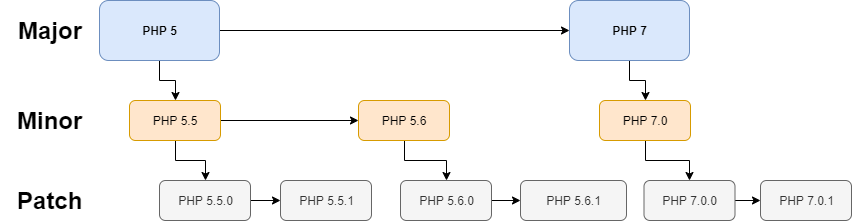
\includegraphics[width=270px]{img/semVer.png}
        \caption{Semantic Versioning am Besipiel von PHP}			
    \end{figure}
\end{frame}

\begin{frame}{ISO/IEC 14764}
    ,,Fahrplan'' zur Migration \nocite{iso/iec_iso/iec/ieee_2006}:
    \begin{itemize}
        \item Anforderungsanalyse und Definition der Migration
        \item Entwicklung von Werkzeugen zur Migration
        \item Entwicklung der angepassten Software
        \item Verifikation der Migration
        \item Support der alten Umgebung
    \end{itemize}
\end{frame}


	
	\section{Ziele von PHP7}
	\begin{frame} {Arten von Änderungen}
	\begin{itemize}
		\item Abwärtsinkompatible Änderungen
		\item Veraltete Funktionen
		\item Geänderte Funktionen
		\item Neue Funktionen
		\item Entfernte Erweiterungen
	\end{itemize}
	\end{frame}

	\begin{frame} {Abwärtsinkompatible Änderungen}
		\textbf{Indirekter Variablenzugriff} \nocite{php_group_php:_nodate-1} \\
		Ausdruck: \$foo$\rightarrow$\$bar['baz']
		\begin{exampleblock}{Interpretation in PHP 5}
			\$foo$\rightarrow$\alert{\$bar['baz']}
		\end{exampleblock}{}
		\begin{exampleblock}{Interpretation in PHP 7}
			\alert{\$foo$\rightarrow$\$bar}['baz']
		\end{exampleblock}{}
	\end{frame}

	\begin{frame}[fragile]{Geänderte Funktionen}
        \textbf{Implizite Konstruktoren} \nocite{morrison_php:_2014}\\
        \begin{lstlisting}
        <?php
        class foo {
          function foo($a) {
            echo("Instance Created");
          }
        }
        ?>
        \end{lstlisting}
    \end{frame}
    
    \begin{frame}[fragile]{Neue Funktionen}
        \textbf{Anonyme Klassen}\\
        \begin{lstlisting}
        <?php
        $foo = new class {
          public function bar() {
            echo("Hello World");
          }
        }

        $foo->bar();
        ?>
        \end{lstlisting}
    \end{frame}

    \begin{frame}[fragile]{Entfernte Erweiterungen}
        \textbf{mysql} \nocite{oracle_mysql_nodate}\\
        \begin{itemize}
            \item keine \alert{Prepared Statements}
            \item Weiterentwicklung aufgegeben
            \item modernere Alternativen
        \end{itemize}  
    \end{frame}

    \begin{frame}{Ziele}
        \begin{itemize}
            \item Erhöhung der Sicherheit
            \item Verständlichkeit des Codes
            \item Höhere Ausführungsgeschwindigkeit
        \end{itemize}  
    \end{frame}
	
	\section{Geeignete Mittel}
	
    \begin{frame}[fragile] {Manuelle Erkennung}
        \textbf{Probleme bei komplexen Strukturen:}
		\begin{lstlisting}
            <?php
            switch(1) {
              default:
                echo("Never evaluated");
                break;
              default:
                echo("Evaluated")
                break;
            }
            ?>
        \end{lstlisting}
    \end{frame}
    
    \begin{frame} {Automatisierte Erkennung}
        \textbf{Vorteile:}
        \begin{itemize}
            \item Erkennung komplexen Codes
            \item Beliebige Projektgröße
            \item Abschätzung über den Aufwand möglich
            \item Bericht als Arbeitsplan
        \end{itemize}
    \end{frame}

    \begin{frame} {Versionsverwaltung}
        \textbf{Vorteile:}
        \begin{itemize}
            \item Protokollierte Änderungen
            \item Historische Versionen zurückverfolgbar
            \item Einfache Bearbeitung durch mehrere Personen
            \item Wartung alter Versionen weiter möglich
        \end{itemize}
    \end{frame}
    
    \begin{frame} {Historischer Code}
        \begin{columns}[T,onlytextwidth]
            \column{0.5\textwidth}
                \textbf{Lokale Umgebungen}
                \begin{itemize}
                    \item Unabhängige Installation
                    \item keine Abhängigkeiten
                    \item keine Versionsverwaltung
                \end{itemize}
            \column{0.5\textwidth}
                \textbf{Docker-Integration} \nocite{anderson_docker_2015}
                \begin{itemize}
                    \item Zentrale Konfiguration
                    \item komplexes Ökosystem
                    \item Versionsverwaltung per \emph{git}
                \end{itemize}
          \end{columns}
    \end{frame}

	\section{Migration}
	\begin{frame} {Anforderungsanalyse}
    \begin{table}
        \centering
        \caption{Anteil zu migrierender Codeteile an der gesamten Codebasis}
        \label{tab:migrationPercentage}
        \begin{tabular}{llll}
                            & Gesamt & Betroffen & Anteil   \\
        \textbf{Dateien}    & 5732   & 690       & 12,04\%  \\
        \textbf{Codezeilen} & 596198 & 1431      & 0,24\%  
        \end{tabular}
    \end{table}
\end{frame}

\begin{frame} {Anforderungsanalyse}
    \begin{figure}
        \begin{tikzpicture}
            \pie [rotate = 0, sum=1425]
            {722/mysql,
             547/Implizite Konstruktoren, 
             86/func\_get\_args,
             21/foreach,
             20/Variablenzugriff,
             35/Andere}
        \end{tikzpicture}
    \end{figure}
\end{frame}

\begin{frame} {Entwicklung von Werkzeugen zur Migration}
    \begin{itemize}
        \item Weiterentwicklung von \emph{php7mar}
        \item Einführung von Docker
        \item Konfiguration von \emph{XDebug}
    \end{itemize}
\end{frame}

\begin{frame}[fragile] {Migration der Software}
    \begin{lstlisting}[language=php]
    //veralteter Aufruf von mysql
    $result = mysql_query($query);
    if(!$result) $output .= mysql_error();
    \end{lstlisting}
    \begin{lstlisting}
    //Ersatz durch mysqli
    $result = mysqli_query($db_link, $query);
    if(!$result) $output .= mysqli_error($db_link);
    \end{lstlisting}
\end{frame}

\begin{frame}[fragile] {Migration der Software}
    \begin{lstlisting}[language=php]
    <?php
    class order {
      function __construct($order_id) {
        $this->order($order_id);
      }

      function order($order_id) {
        print($order_id);
      }
    }
    ?>
    \end{lstlisting}
\end{frame}

\begin{frame}{Verifikation}
    \begin{itemize}
        \item Manuelles Testen
        \item Monitoring mittels \emph{New Relic}
        \item keine Unit Tests
    \end{itemize}
\end{frame}

\begin{frame}{Support der alten Umgebung}
    \begin{itemize}
        \item Für hauseigene Software weniger relevant
        \item Parallelbetrieb während Übergangszeit
        \item Historischer Code weiter in Versionsverwaltung
    \end{itemize}
\end{frame}	

	\section{Auswertung}
	\begin{frame}{Ziele}
    \textbf{Sicherheit:}
    \begin{itemize}
        \item Entfernung von \emph{mysql}
        \item Entfernung potentieller Risiken
    \end{itemize}
    \textbf{Klarheit des Codes:}
    \begin{itemize}
        \item Einheitliche Konstruktoraufrufe
        \item Einheitliche Variablenaufrufe
    \end{itemize}
\end{frame}

\begin{frame}{Ziele}
    \textbf{Geschwindigkeit:}
    \begin{figure}
        \begin{tikzpicture}
          \begin{axis}[
            mlineplot,
            xlabel={Zeit in h},
            ylabel={Ausführungszeit in ms},
            ymin = 0,
            ymax = 90,
            width=0.9\textwidth,
            height=6cm,
          ]
    
            \addplot coordinates {(0,66.1) (1, 66.1) (2, 62.3) (3, 79.4) (4, 53.3) (5, 66.4) (6,63.6) (7,65.8) (8,67.1) (9,66) (10,66.4) (11,66.9) (12,66.3) (13,66.5) (14,65.9) (15,66.2) (16,63.9) (17,65.5) (18,67.6) (19,67.4) (20,66.5) (21,67.1) (22,67) (23,66) };
            \addplot coordinates {(0,43.3) (1, 41.1) (2, 40.7) (3, 67) (4, 27.5) (5, 38.9) (6,43) (7,44.6) (8,43.9) (9,42.8) (10,43) (11,41.6) (12,41.7) (13,41) (14,41.5) (15,43.1) (16,44.9) (17,42.4) (18,43.5) (19,44.4) (20,44.9) (21,45.5) (22,45.8) (23,45.1) };

            \legend{PHP5, PHP7}
          \end{axis}
        \end{tikzpicture}
      \end{figure}
\end{frame}

	\section{Ausblick}
	\include{sections/Section6}

	\begin{frame}[allowframebreaks]{Referenzen}
		\bibliography{Bibliography}
		\bibliographystyle{alpha}	  
	  \end{frame}
\end{document}